% Options for packages loaded elsewhere
\PassOptionsToPackage{unicode=true}{hyperref}
\PassOptionsToPackage{hyphens}{url}
%
\documentclass[
]{book}
\usepackage{lmodern}
\usepackage{amssymb,amsmath}
\usepackage{ifxetex,ifluatex}
\ifnum 0\ifxetex 1\fi\ifluatex 1\fi=0 % if pdftex
  \usepackage[T1]{fontenc}
  \usepackage[utf8]{inputenc}
  \usepackage{textcomp} % provides euro and other symbols
\else % if luatex or xelatex
  \usepackage{unicode-math}
  \defaultfontfeatures{Scale=MatchLowercase}
  \defaultfontfeatures[\rmfamily]{Ligatures=TeX,Scale=1}
\fi
% Use upquote if available, for straight quotes in verbatim environments
\IfFileExists{upquote.sty}{\usepackage{upquote}}{}
\IfFileExists{microtype.sty}{% use microtype if available
  \usepackage[]{microtype}
  \UseMicrotypeSet[protrusion]{basicmath} % disable protrusion for tt fonts
}{}
\makeatletter
\@ifundefined{KOMAClassName}{% if non-KOMA class
  \IfFileExists{parskip.sty}{%
    \usepackage{parskip}
  }{% else
    \setlength{\parindent}{0pt}
    \setlength{\parskip}{6pt plus 2pt minus 1pt}}
}{% if KOMA class
  \KOMAoptions{parskip=half}}
\makeatother
\usepackage{xcolor}
\IfFileExists{xurl.sty}{\usepackage{xurl}}{} % add URL line breaks if available
\IfFileExists{bookmark.sty}{\usepackage{bookmark}}{\usepackage{hyperref}}
\hypersetup{
  pdftitle={mmir: An R-package for Simple Biological Metric Calculations},
  pdfauthor={Zachary M. Smith},
  hidelinks,
}
\urlstyle{same} % disable monospaced font for URLs
\usepackage{color}
\usepackage{fancyvrb}
\newcommand{\VerbBar}{|}
\newcommand{\VERB}{\Verb[commandchars=\\\{\}]}
\DefineVerbatimEnvironment{Highlighting}{Verbatim}{commandchars=\\\{\}}
% Add ',fontsize=\small' for more characters per line
\usepackage{framed}
\definecolor{shadecolor}{RGB}{248,248,248}
\newenvironment{Shaded}{\begin{snugshade}}{\end{snugshade}}
\newcommand{\AlertTok}[1]{\textcolor[rgb]{0.94,0.16,0.16}{#1}}
\newcommand{\AnnotationTok}[1]{\textcolor[rgb]{0.56,0.35,0.01}{\textbf{\textit{#1}}}}
\newcommand{\AttributeTok}[1]{\textcolor[rgb]{0.77,0.63,0.00}{#1}}
\newcommand{\BaseNTok}[1]{\textcolor[rgb]{0.00,0.00,0.81}{#1}}
\newcommand{\BuiltInTok}[1]{#1}
\newcommand{\CharTok}[1]{\textcolor[rgb]{0.31,0.60,0.02}{#1}}
\newcommand{\CommentTok}[1]{\textcolor[rgb]{0.56,0.35,0.01}{\textit{#1}}}
\newcommand{\CommentVarTok}[1]{\textcolor[rgb]{0.56,0.35,0.01}{\textbf{\textit{#1}}}}
\newcommand{\ConstantTok}[1]{\textcolor[rgb]{0.00,0.00,0.00}{#1}}
\newcommand{\ControlFlowTok}[1]{\textcolor[rgb]{0.13,0.29,0.53}{\textbf{#1}}}
\newcommand{\DataTypeTok}[1]{\textcolor[rgb]{0.13,0.29,0.53}{#1}}
\newcommand{\DecValTok}[1]{\textcolor[rgb]{0.00,0.00,0.81}{#1}}
\newcommand{\DocumentationTok}[1]{\textcolor[rgb]{0.56,0.35,0.01}{\textbf{\textit{#1}}}}
\newcommand{\ErrorTok}[1]{\textcolor[rgb]{0.64,0.00,0.00}{\textbf{#1}}}
\newcommand{\ExtensionTok}[1]{#1}
\newcommand{\FloatTok}[1]{\textcolor[rgb]{0.00,0.00,0.81}{#1}}
\newcommand{\FunctionTok}[1]{\textcolor[rgb]{0.00,0.00,0.00}{#1}}
\newcommand{\ImportTok}[1]{#1}
\newcommand{\InformationTok}[1]{\textcolor[rgb]{0.56,0.35,0.01}{\textbf{\textit{#1}}}}
\newcommand{\KeywordTok}[1]{\textcolor[rgb]{0.13,0.29,0.53}{\textbf{#1}}}
\newcommand{\NormalTok}[1]{#1}
\newcommand{\OperatorTok}[1]{\textcolor[rgb]{0.81,0.36,0.00}{\textbf{#1}}}
\newcommand{\OtherTok}[1]{\textcolor[rgb]{0.56,0.35,0.01}{#1}}
\newcommand{\PreprocessorTok}[1]{\textcolor[rgb]{0.56,0.35,0.01}{\textit{#1}}}
\newcommand{\RegionMarkerTok}[1]{#1}
\newcommand{\SpecialCharTok}[1]{\textcolor[rgb]{0.00,0.00,0.00}{#1}}
\newcommand{\SpecialStringTok}[1]{\textcolor[rgb]{0.31,0.60,0.02}{#1}}
\newcommand{\StringTok}[1]{\textcolor[rgb]{0.31,0.60,0.02}{#1}}
\newcommand{\VariableTok}[1]{\textcolor[rgb]{0.00,0.00,0.00}{#1}}
\newcommand{\VerbatimStringTok}[1]{\textcolor[rgb]{0.31,0.60,0.02}{#1}}
\newcommand{\WarningTok}[1]{\textcolor[rgb]{0.56,0.35,0.01}{\textbf{\textit{#1}}}}
\usepackage{longtable,booktabs}
% Allow footnotes in longtable head/foot
\IfFileExists{footnotehyper.sty}{\usepackage{footnotehyper}}{\usepackage{footnote}}
\makesavenoteenv{longtable}
\usepackage{graphicx,grffile}
\makeatletter
\def\maxwidth{\ifdim\Gin@nat@width>\linewidth\linewidth\else\Gin@nat@width\fi}
\def\maxheight{\ifdim\Gin@nat@height>\textheight\textheight\else\Gin@nat@height\fi}
\makeatother
% Scale images if necessary, so that they will not overflow the page
% margins by default, and it is still possible to overwrite the defaults
% using explicit options in \includegraphics[width, height, ...]{}
\setkeys{Gin}{width=\maxwidth,height=\maxheight,keepaspectratio}
\setlength{\emergencystretch}{3em} % prevent overfull lines
\providecommand{\tightlist}{%
  \setlength{\itemsep}{0pt}\setlength{\parskip}{0pt}}
\setcounter{secnumdepth}{5}
% Redefines (sub)paragraphs to behave more like sections
\ifx\paragraph\undefined\else
  \let\oldparagraph\paragraph
  \renewcommand{\paragraph}[1]{\oldparagraph{#1}\mbox{}}
\fi
\ifx\subparagraph\undefined\else
  \let\oldsubparagraph\subparagraph
  \renewcommand{\subparagraph}[1]{\oldsubparagraph{#1}\mbox{}}
\fi

% Set default figure placement to htbp
\makeatletter
\def\fps@figure{htbp}
\makeatother


\title{mmir: An R-package for Simple Biological Metric Calculations}
\usepackage{etoolbox}
\makeatletter
\providecommand{\subtitle}[1]{% add subtitle to \maketitle
  \apptocmd{\@title}{\par {\large #1 \par}}{}{}
}
\makeatother
\subtitle{Northeast Aquatic Biologists Conference 2020}
\author{Zachary M. Smith}
\date{March 5th, 2020}

\begin{document}
\maketitle

{
\setcounter{tocdepth}{1}
\tableofcontents
}
\hypertarget{title-page}{%
\chapter{Title Page}\label{title-page}}


\includegraphics[width=5.20833in,height=\textheight]{images/mmir_hex-sticker.png}

\hypertarget{introduction}{%
\chapter{Introduction}\label{introduction}}

\hypertarget{objective}{%
\section{Objective}\label{objective}}

\begin{itemize}
\tightlist
\item
  Demonstrate the functionality provided by the \textbf{mmir} R-package for calculating biological metrics for the development and/or use in an MMI or IBI.
\end{itemize}

\hypertarget{what-is-an-mmi}{%
\section{What is an MMI?}\label{what-is-an-mmi}}

\begin{itemize}
\tightlist
\item
  Multi-Metric Indices (MMIs) or Indices of Biotic Integrity (IBIs) are models that summarize multiple aspects of a biological community of interest (e.g., richness, diversity, relative abundance, tolerance, and functional feeding group) into a single numeric or categorical value representing ecological condition.

  \begin{itemize}
  \tightlist
  \item
    considered a robust measure of water quality becuase it represents more than a snapshot in time
  \item
    have been around for nearly 40 years
  \end{itemize}
\end{itemize}

\hypertarget{need}{%
\section{Need}\label{need}}

\begin{itemize}
\tightlist
\item
  MMIs are widely used by U.S. federal and state agencies to assess water quality but there is no R-package available to simplify and standardize metric calculations.
\end{itemize}

\hypertarget{r-overview}{%
\chapter{R Overview}\label{r-overview}}

\hypertarget{r-packages}{%
\section{R Packages}\label{r-packages}}

\includegraphics{images/r_packages.png}

\hypertarget{r-functions}{%
\section{R Functions}\label{r-functions}}

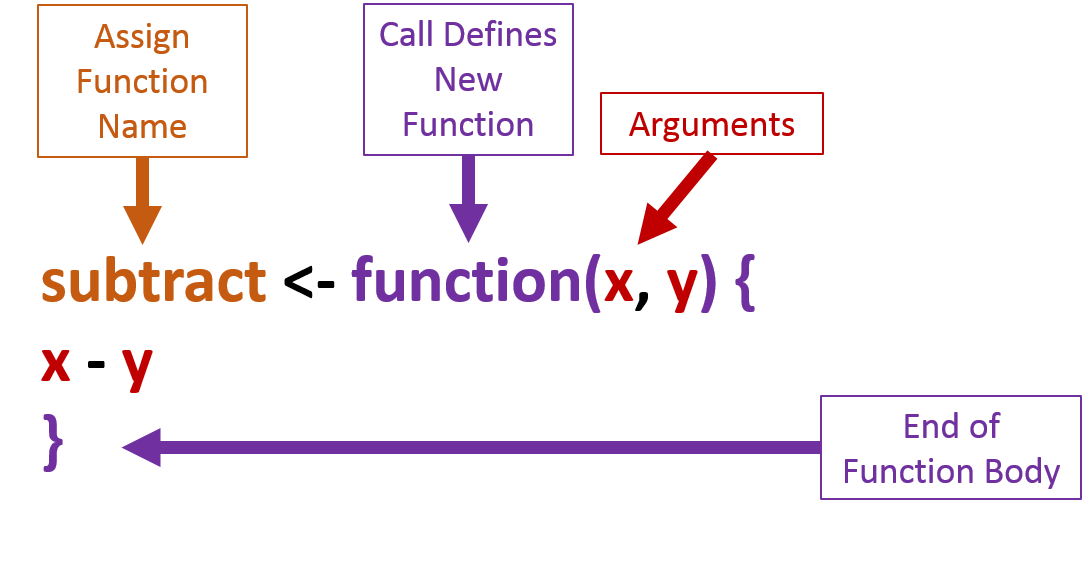
\includegraphics{images/func_structure.png}

\hypertarget{tidyverse}{%
\section{Tidyverse}\label{tidyverse}}

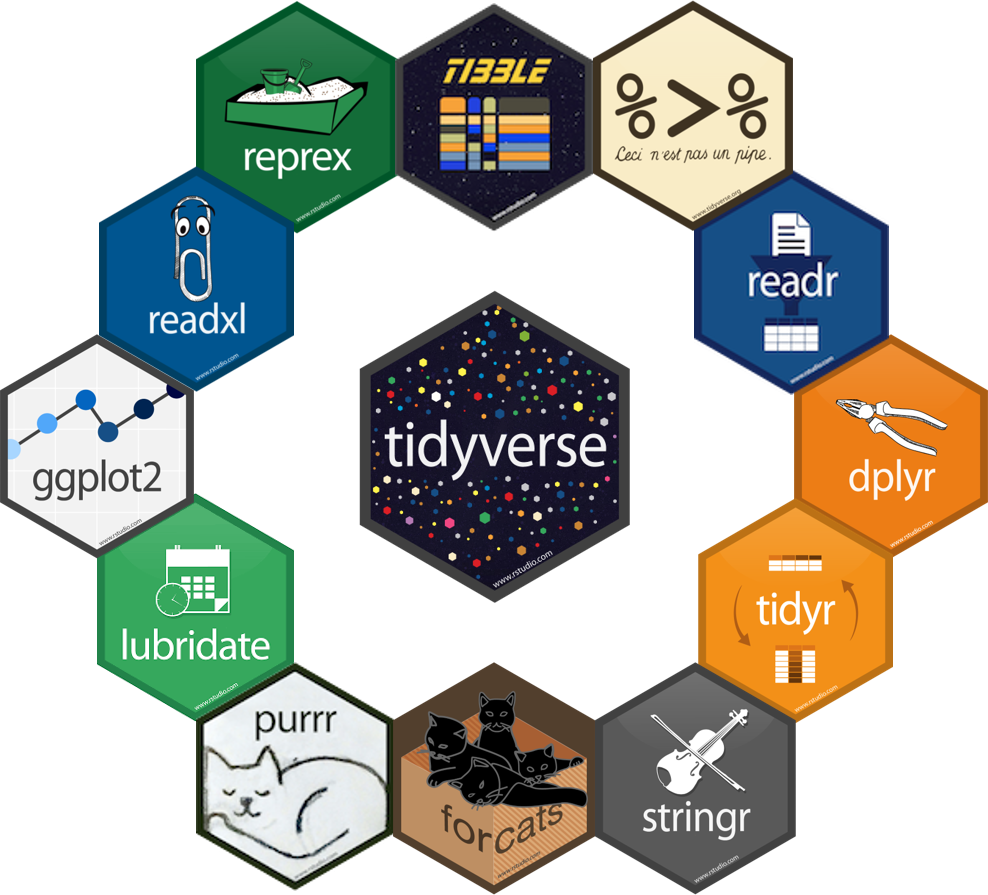
\includegraphics{images/tidyverse_circle.png}

\hypertarget{installation-of-mmir}{%
\chapter{Installation of mmir}\label{installation-of-mmir}}

Install the Multi-Metric Index (MMI) package, \textbf{mmir}, that I am developing from GitHub (\url{https://github.com/zsmith27/mmir}).

\begin{Shaded}
\begin{Highlighting}[]
\NormalTok{devtools}\OperatorTok{::}\KeywordTok{install_github}\NormalTok{(}\StringTok{"zsmith27/mmir"}\NormalTok{)}
\end{Highlighting}
\end{Shaded}

\hypertarget{load-the-package}{%
\section{Load the Package}\label{load-the-package}}

Once \textbf{mmir} is installed, load the package with \texttt{library()}.

\begin{Shaded}
\begin{Highlighting}[]
\KeywordTok{library}\NormalTok{(mmir)}
\end{Highlighting}
\end{Shaded}

\hypertarget{required-data-format}{%
\chapter{Required Data Format}\label{required-data-format}}

Placeholder

\hypertarget{required-data-format-example}{%
\section{Required Data Format Example}\label{required-data-format-example}}

\hypertarget{data-preparation}{%
\section{Data Preparation}\label{data-preparation}}

\hypertarget{metrics}{%
\chapter{Metrics}\label{metrics}}

Placeholder

\hypertarget{metric-function-list}{%
\section{Metric Function List}\label{metric-function-list}}

\hypertarget{metric-function-arguements}{%
\section{Metric Function Arguements}\label{metric-function-arguements}}

\end{document}
